% Chris Hanusa
% chanusa@qc.cuny.edu	
\documentclass[12pt]{article} 

\usepackage{amssymb,amsthm,amsmath,epsfig}

\usepackage{color}
\definecolor{darkblue}{rgb}{0, 0, .4}
\definecolor{grey}{rgb}{.7, .7, .7}

\setlength{\topmargin}{-.5in}
\setlength{\textheight}{9in}
\setlength{\textwidth}{6.5in}
%\setlength{\headheight}{26pt}
%\setlength{\headsep}{2pt}
\setlength{\oddsidemargin}{0in}
\setlength{\evensidemargin}{0in}

\newcommand{\lam}{\lambda}

\usepackage[breaklinks]{hyperref} 
\hypersetup{
    colorlinks=true,
    linkcolor=darkblue,
    anchorcolor=darkblue,
    citecolor=darkblue,
    pagecolor=darkblue,
    urlcolor=darkblue,
    pdftitle={},
    pdfauthor={}
}

\begin{document}
\pagestyle{empty}

%%%%%%%%%%%%%%%%%%%%%%%%%%%%%%%%%%%%%%%%%%%%%%%%%%%%%%%%%%%%%%%%%%%%%%
%%%%%%%%%%%%%%%%%%%%%%%%%%%%%%%%%%%%%%%%%%%%%%%%%%%%%%%%%%%%%%%%%%%%%%

\begin{center}\large 
MATH 634, Spring 2014

{\sc Homework 5}

due 5:00{\sc pm} on Wednesday, February 19.
\end{center}

\noindent
{\em Background reading:} {\em Pearls in Graph Theory}, Section 1.3 and 2.1.

\smallskip\noindent
{\color{red} Follow the posted homework guidelines when completing this assignment.}

\smallskip\noindent
Problems {\bf 5D}, {\bf 5E}, and {\bf 5P} should be typed (or written up) and handed in as class starts on Wednesday 2/19:

\begin{enumerate}
\item[\bf 5D.]  

\begin{itemize}
\item (vertex) coloring of a graph 
\item proper (vertex) coloring of a graph
\item chromatic number of a graph
\item critical graph
\item clique number of a graph
\end{itemize}


\item[\bf 5E.]
%09h4
Sudoku is sooo last decade! Solve this Hashi puzzle.

\begin{center}
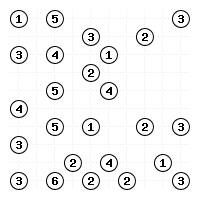
\includegraphics[height=1.5in]{figures/Hashi}
\end{center}
%\item[\bf 5E.]
%%11h2,13h2
%Let $G$ be a connected regular graph with 22 edges.  What are the possible number of vertices that $G$ may have?
{\bf Instructions:}  Draw in lines to connect the circles such that:
\begin{itemize}
\item Lines must be either perfectly vertical or horizontal.
\item Up to two lines may be drawn connecting the same circles.  
\item The lines may not cross.
\item The degree of each vertex is the enclosed number.  
\item The entire graph must be connected.
\end{itemize}
For many more Hashi puzzles and other fun games, visit \newline\url{http://www.menneske.no/hashi/eng/} \& \url{http://www.puzzle-bridges.com/}.



\item[\bf 5P.] 
%12h3, 13h3
% Pearls 1.3.1
Consider a tree $T$ that has only vertices of degree $1$, $2$, and $3$.  Suppose that $T$ has exactly 10 vertices of degree $3$.  Find and prove how many leaves $T$ has.   \newline[{\em Important: Prove your answer for {\bf any} tree $T$ satisfying these conditions.}] 

\end{enumerate}


\end{document}














